%%%%%%%%%%%%%%%%%%%%%%%%%%%%%%%%%%%%%%%%%%%%%%%%%%%%%%%%%%%%%%%%%%%%%%%%%%%%%%%%%%%%%%%%%%%%%%%%%%%%%%%%%%%%%%%%%%%%%%%%%%%%%%%%%%%%%%%%%%%%%%%%%%%%%%
% 20141009 - Introduction to Operating Systems VO
%%%%%%%%%%%%%%%%%%%%%%%%%%%%%%%%%%%%%%%%%%%%%%%%%%%%%%%%%%%%%%%%%%%%%%%%%%%%%%%%%%%%%%%%%%%%%%%%%%%%%%%%%%%%%%%%%%%%%%%%%%%%%%%%%%%%%%%%%%%%%%%%%%%%%%

%fancyhdr
\lhead{IOS VO} 
\rhead{2014-10-09}

%%%%%%%%%%%%%%%%%%%%%%%%%%%%%%%%%%%%%%%%%%%%%%%%%%%%%%%%%%%%%%%%%%%%%%%%%%%%%%%%%%%%%%%%%%%%%%%%%%%%%%%%%%%%%%%%%%%%%%%%%%%%%%%%%%%%%%%%%%%%%%%%%%%%%%

\par{
	\noindent
	What we want:
	\begin{figure}[H]
		\centering
		\begin{tikzpicture}
			\node[draw, minimum width = 2cm, minimum height = 8cm] (physmem) at (0, 0) {};
			\node[left = 0 of physmem.south west] (physmem_0) {0};
			\node[left = 0 of physmem.north west] (physmem_max) {max};
			\node[below = 0.25 of physmem.south] (physmem_t) {phys. memory};

			\foreach \i [count = \ii from 1] in {A, B}{
				\node[draw, right = \ii * 4 of physmem.north east, minimum width = 0.25cm, minimum height = 0.5cm] (reg_proc\i) {};
				\node[above = 0 of reg_proc\i] (reg_proc\i_t) {reg};
				\node[draw, right = 0.25 of reg_proc\i.east, minimum width = 2cm, minimum height = 0.5cm] (stack_proc\i) {\footnotesize{Stack}};
				\node[draw, below = 1.5 of stack_proc\i, minimum width = 2cm, minimum height = 0.5cm] (heap_proc\i) {\footnotesize{Heap}};
				\node[draw, below = -0.015 of heap_proc\i.south, minimum width = 2cm, minimum height = 1cm] (globals_proc\i) {\footnotesize{Globals}};
				\node[draw, below = -0.015 of globals_proc\i.south, minimum width = 2cm, minimum height = 3cm] (code_proc\i) {\footnotesize{Code}};
				\draw (stack_proc\i.north west) -- (stack_proc\i.north east) -- (code_proc\i.south east) -- (code_proc\i.south west) -- (stack_proc\i.north west);
				\node[below = 0.25 of code_proc\i.south] (proc\i_t) {process \i};
				\draw[<-, >=stealth] (code_proc\i.west) -- ++(-0.5, 0);
				\draw[->, >=stealth] (stack_proc\i.south) -- ++(0, -0.25);
				\draw[->, >=stealth] (heap_proc\i.north) -- ++(0, 0.25);
				\draw[dotted] (code_proc\i.west) ++(-0.25, 0) -- ++(0, -1.75);
			}
			\draw[dotted] (code_procA.west) ++(-0.25, -1.75) -- ++(4, 0);
			\draw[<-, >=stealth] (code_procB.west) ++(-0.75, -1.75) -- ++(0, -1) node[below] {\footnotesize{context switch}};
		\end{tikzpicture}
		\caption{Each process thinks it owns the whole memory.}
		\label{fig:concurrencymem}
	\end{figure}
	\noindent
	Each process has its own virtual memory which is loaded whenever a context switch is performed. \textit{Concurrency} (competing for resources, time sharing) $\not=$ \textit{Parallelism} (truely parallel, multiple processors). \textit{Spatial isolation} is necessary to enable concurrency.
}

\par{
	\noindent\underline{Data structures:}
	\par{
		\noindent
		2 Goals:
		\parskip0pt\begin{enumerate}
			\item{Abstraction: table, list, tree, graph, \ldots}
			\item{Safety: only accessing memory we have declared, memory access as specified.}
		\end{enumerate}
	}
	\par{
		\noindent
		2 levels where we can have safety:
		\begin{figure}[H]
			\centering
			\begin{tikzpicture}
				\node[draw, minimum height = 2cm, minimum width = 2cm, text width = 2cm, text centered] (gc) at (1, 0) {Garbage Collector};
				\node[draw, right = 1 of gc, minimum height = 1cm, minimum width = 4cm] (range_checking) {range checking};
				\draw[] (gc.north west) ++(-0.5, 0.5) -- ++(12, 0);
				\node[draw, above = 2 of range_checking, minimum height = 1cm, minimum width = 4cm] (type_checking) {type checking};

				\node[right = 2 of range_checking] (runtime_t) {runtime};
				\node[right = 2 of type_checking] (compiletime_t) {compile time};

				\draw[<-, >=stealth] (type_checking.north east) -- ++(0.5, 0.5) node[right, text width = 4cm] {\footnotesize{has to be strong enough, \textit{static typing}}};
			\end{tikzpicture}
			\caption{safety levels}
			\label{fig:safetylevels}
		\end{figure}
	}
	\par{
		\noindent
		Unless all accesses use constants as indices, in general no compiler can perform a range check at compile time. At some point there is a limit. E.g. \texttt{i = 10; a[i];} is recognized by some compilers. \newline
		If you do not allow dynamic allocation, your language does not allow to write a program which accesses memory outside (type and range checks required of course!). \newline
		Suppose a \texttt{free} mechanism: you could free something and access it afterwards, or you could do \texttt{free(obj);} which creates a \textit{dangling pointer}, and do \texttt{obj.field = 1;} afterwards.
	}
	\par{
		\noindent
		\begin{minipage}{0.45\textwidth}
			\setlength{\parskip}{12pt plus2pt minus2pt}
			\par{
				\noindent\underline{Arrays:}
				\begin{lstlisting}[language = C, frame = none]
	int a[3];
				\end{lstlisting}
				The advantage of the contiguous layout in memory: constant time access.\newline
				The big drawback of the contiguous layout in memory: fragmentation. \newline
				3 ingredients of fragmentation:
				\parskip0pt\begin{enumerate}
					\item{contiguously allocated memory gives us constant time access (could be splitted as well)}
					\item{blocks of different size}
					\item{the order of deallocation is not equal to the order of allocation}
				\end{enumerate}
				In the worst case, there is a 50/50 allocation present. If we then want to allocate a big chunk of memory, it is not possible without some reordering.
			}
			\par{
				\noindent\underline{Records:}
				\begin{lstlisting}[language = C, frame = none]
	struct rec {
		int i;
		struct rec *r;
	};
				\end{lstlisting}
				The advantages of the contiguous layout in memory:
				\parskip0pt\begin{itemize}
					\item{constant time access (even faster than the array access because the offsets can be computed at compile time)}
					\item{no fragmentation (if the implementer knows what s/he is doing)}
				\end{itemize}
				The disadvantage is the fact that the access complexity is not constant but linear in the size of the list.
			}
		\end{minipage}%
		\hfill
		\begin{minipage}{0.45\textwidth}
			\begin{figure}[H]
				\centering
				\begin{tikzpicture}
					\def\cellheight{0.65cm}
					\tikzset{memcontcell/.style = {draw, minimum height = \cellheight, minimum width = 2cm}};
					\tikzset{memposcell/.style = {minimum height = \cellheight}};
					\tikzset{brace/.style = {decoration = {brace, mirror, raise = 4ex}, decorate}}

					\node[memposcell] (mem_pos0) at (0, 0) {0};
					\node[memcontcell, right = -0.015 of mem_pos0] (mem_cont0) {\texttt{3 (= i)}};

					\foreach \i [count = \ii from 0] in {1, ..., 8}{
						\node[memposcell, above = -0.015 of mem_pos\ii] (mem_pos\i) {\i};
					}

					\node[memcontcell, above = -0.015 of mem_cont0] (mem_cont1) {\texttt{3 (= r)}};
					\node[memcontcell, above = -0.015 of mem_cont1] (mem_cont2) {};
					\node[memcontcell, above = -0.015 of mem_cont2] (mem_cont3) {\texttt{4}};
					\node[memcontcell, above = -0.015 of mem_cont3] (mem_cont4) {\texttt{0}};
					\node[memcontcell, above = -0.015 of mem_cont4] (mem_cont5) {};
					\node[memcontcell, above = -0.015 of mem_cont5] (mem_cont6) {\texttt{5}};
					\node[memcontcell, above = -0.015 of mem_cont6] (mem_cont7) {\texttt{2}};
					\node[memcontcell, above = -0.015 of mem_cont7] (mem_cont8) {\texttt{6}};

					\node[draw, minimum height = 5cm, minimum width = 2cm, above = -0.015 of mem_cont8] (mem_contdots) {\ldots};
					\node[memcontcell, above = -0.015 of mem_contdots] (mem_contmax) {};
					\node[memposcell, left = -0.015 of mem_contmax] (mem_posmax) {max};
					\node[above = 0 of mem_contmax] (abstract_memory_t) {abstract memory};

					\draw[->, >=stealth] (mem_cont1.east) -- ++(0.5, 0) -- ++(0, \cellheight * 2) -- (mem_cont3.east);
					\draw[brace] (mem_cont0.south east) -- node[right, xshift = 6ex] {\texttt{struct rec}} (mem_cont1.north east);
					\draw[brace] (mem_cont3.south east) -- node[right, xshift = 6ex] {\texttt{struct rec}} (mem_cont4.north east);
					\draw[brace] (mem_cont6.south east) -- node[right, xshift = 6ex] {\texttt{int a[3]}} (mem_cont8.north east);
					\draw[<-, >=stealth, dotted] (mem_cont4.east) -- ++(1, 0.75) node[right] {zero: end of linked list};
				\end{tikzpicture}
				\caption{Arrays and records in the memory}
				\label{fig:arraysrecordsmem}
			\end{figure}
		\end{minipage}%
	}
	\clearpage
	\par{
		\noindent
		The only other option (to use contiguous allocation):
		\begin{center}
			\textbf{Construct data structures out of pointers}.
		\end{center}
		If we just allocate a billion of \texttt{struct rec} (which actually all have the same size), there is no fragmentation.
	}
}

\par{
	\noindent\underline{Memory Hierarchy:}
	\begin{figure}[H]
		\centering
		\begin{tikzpicture}	
			\tikzset{pyramidenode/.style = {draw, trapezium, trapezium left angle = 60, trapezium right angle = 60, minimum height = 1cm, text centered}}
			\node (throughput_t) at (0, 0) {\textit{throughput}};
			\node[above = 0.15 of throughput_t.north] (min_t) {min};
			\node[above = 6 of min_t] (max_t) {max};
			\draw[->, >=stealth] (min_t.north east) -- (max_t.south east);

			\node[pyramidenode, above right = 0 and 4 of min_t, text width = 3.574cm] (cloud) {Cloud};
			\node[pyramidenode, above = -0.015 of cloud, text width = 3.35cm] (storage) {Storage};
			\node[pyramidenode, above = -0.015 of storage, text width = 2.6cm] (mainmemory) {Main Memory}; 
			\node[pyramidenode, above = -0.015 of mainmemory, text width = 1.6cm] (caches) {Caches};
			\node[pyramidenode, above = -0.015 of caches, text width = 1.1125cm] (register) {Reg};
			\node[draw, above = -0.015 of register, regular polygon, regular polygon sides = 3, minimum width = 1cm, text width = 0.6cm] {};

			% invisible nodes to curve pointers
			\node[left = 1 of caches.west] (caches_left) {};
			\node[left = 0.5 of mainmemory.west] (mainmemory_left) {};
			\draw[<->, >=stealth] (caches.west) .. controls (caches_left) and (mainmemory_left) .. (mainmemory.west) node[above left = 0.25 and 0.4] {\tiny{Hardware}};

			\node[right = 1.5 of register.east] (register_right) {};
			\node[right = 0.5 of mainmemory.east] (mainmemory_right) {};
			\draw[<->, >=stealth] (register.east) .. controls (register_right) and (mainmemory_right) .. (mainmemory.east) node[above right = 0.75 and 0.4] {\tiny{Compiler/Interpreter}};

			\node[right = 0.5 of storage.east] (storage_right) {};
			\draw[->, >=stealth] (mainmemory.east) .. controls (mainmemory_right) and (storage_right) .. (storage.east) node[above right = 0.25 and 0.4] {\tiny{OS}};

			\node[right = 0.5 of cloud.east] (cloud_right) {};
			\draw[->, >=stealth] (storage.east) .. controls (storage_right) and (cloud_right) .. (cloud.east) node[above right = 0.25 and 0.4] {\tiny{Services}};

			\node[right = 0.5 of mainmemory.east] (memorymanagement) {\tiny{Memory management}};

			\node[right = 8.5 of throughput_t] (latency_t) {\textit{latency}};
			\node[above = 0.15 of latency_t.north] (lat_max_t) {max};
			\node[above = 6 of lat_max_t] (lat_min_t) {min};
			\draw[<-, >=stealth] (lat_max_t.north east) -- (lat_min_t.south east);

			\node[right = 0.25 of latency_t] (capacity_t) {\textit{capacity}};
			\node[above = 0.15 of capacity_t.north] (cap_max_t) {max};
			\node[above = 6 of cap_max_t] (cap_min_t) {min};
			\draw[<-, >=stealth] (cap_max_t.north east) -- (cap_min_t.south east);

			\node[right = 0.25 of capacity_t] (volatility_t) {\textit{volatility}};
			\node[above = 0.15 of volatility_t.north] (vol_min_t) {min};
			\node[above = 6 of vol_min_t] (vol_max_t) {max};
			\draw[->, >=stealth] (vol_min_t.north east) -- (vol_max_t.south east);
 		\end{tikzpicture}
 		\caption{Memory hierarchy}
 		\label{fig:memhierarchy}
	\end{figure}
	\par{
		\noindent
		\textit{Services}: Dropbox, Google Cloud, \ldots
	}
}

\clearpage
\par{
	\noindent\underline{Caches:}
	\begin{figure}[H]
		\centering
		\begin{tikzpicture}
			\node[draw] (legendX) at (0, 0) {X};
			\node[right = 0 of legendX] (legendX_descr) {\ldots not used};

			\tikzset{cacheentry/.style = {draw, minimum width = 1.5cm, minimum height = 1cm}}
			\node[cacheentry, above = 0.5 of legendX_descr] (cacheentry0) {X};
			\node[left = 0 of cacheentry0] (cacheentry0_nr) {0};
			\node[cacheentry, above = -0.015 of cacheentry0] (cacheentry1) {X};
			\node[left = 0 of cacheentry1] (cacheentry1_nr) {1};

			\foreach \i [count = \ii from 1] in {2, 3, 4}{
				\node[cacheentry, above = -0.015 of cacheentry\ii] (cacheentry\i) {};
				\node[left = 0 of cacheentry\i] (cacheentry\i_nr) {\i};
			}
			\node[cacheentry, above = -0.015 of cacheentry4] (cacheentry5) {X};
			\node[left = 0 of cacheentry5] (cacheentry5_nr) {5};

			\node[draw, minimum width = 2cm, minimum height = 1cm, right = 3 of cacheentry1.north east] (address0) {};
			\node[draw, minimum width = 2cm, minimum height = 1cm, above = -0.015 of address0] (address1) {2-4};
			\node[draw, minimum width = 2cm, minimum height = 1.5cm, above = -0.015 of address1] (address2) {};
			\node[draw, minimum width = 3cm, minimum height = 1cm, right = -0.015 of address0] (cacheline0) {};
			\node[draw, minimum width = 1cm, minimum height = 1cm, right = -0.015 of address1] (cacheline1_1) {\tiny{(2)}};
			\node[draw, minimum width = 1cm, minimum height = 1cm, right = -0.015 of cacheline1_1] (cacheline1_2) {\tiny{(3)}};
			\node[draw, minimum width = 1cm, minimum height = 1cm, right = -0.015 of cacheline1_2] (cacheline1_3) {\tiny{(4)}};
			\node[draw, minimum width = 3cm, minimum height = 1.5cm, right = -0.015 of address2] (cacheline2) {};

			\node[above = 0.5 of address2.north] (address_t) {\textit{address}};
			\node[above = 0.5 of cacheline2.north] (cacheline_t) {\textit{cache line}};
			\draw[->, >=stealth] (cacheline_t.south) -- (cacheline2.north);
			\draw[->, >=stealth] (address_t.south) -- (address2.north);
			\draw[->, >=stealth] (cacheline2.north east) ++(0.5, 0) -- ++(0, -3.5cm); 

			\tikzset{brace/.style = {decoration = {brace, mirror, raise = 1ex}, decorate}}
			\draw[brace] (cacheentry2.south east) -- node[right] (brace_middle) {} (cacheentry4.north east);
			\node[right = 1 of brace_middle] (brace_middle_r) {};
			\node[left = 1 of address1] (address1_l) {};
			\draw[<-, >=stealth] (address1.west) .. controls (address1_l) and (brace_middle_r) .. (brace_middle.east) node[above right] {\textit{cache hit}};
		\end{tikzpicture}
		\caption{Caches}
		\label{fig:caches}
	\end{figure}
	\par{
		\noindent
		\par{\noindent Why is caching beneficial? Checking and searching in the cache and not the main memory is much faster.}
		\par{
			\noindent
			What motivates a cache? \textit{Temporal locality}: access of a given memory location is likely to be followed by an access of the same location in the near future. Examples are looping und sequentiality.
		}
		\par{
			\noindent
			What motivates a cache line? \textit{Spatial locality}: access of a given memory location is likely to be followed by a location nearby (local memory neighbor location). This is especially beneficial for sequential code and may be bad for parallel code. An example is the linearity of data structures  in the memory.
		}
		\par{
			\noindent
			An example where cache lines are bad for parallel code: if 2 threads have two variables and align them in the cache line like in Figure~\ref{fig:cacheline_bad}. This is the worst case because the cache line has to be replaced every time.
			\begin{figure}[H]
				\centering
				\begin{tikzpicture}
					\tikzset{brace/.style = {decoration = {brace, mirror, raise = 1ex}, decorate}}
					\node[draw, minimum height = 1cm, minimum width = 1.5cm] (cacheline2) {\tiny{(2)} \normalsize X};
					\node[draw, minimum height = 1cm, minimum width = 1.5cm, right = -0.015 of cacheline2] (cacheline3) {\tiny{(3)}};
					\node[draw, minimum height = 1cm, minimum width = 1.5cm, right = -0.015 of cacheline3] (cacheline4) {\tiny{(4)} \normalsize X};
				\end{tikzpicture}
				\caption{Example of \textit{false sharing}}
				\label{fig:cacheline_bad}
			\end{figure}
		}
		\clearpage
		\par{
			\noindent
			There are two extreme design choices when it comes to cache design:
			\parskip0pt\begin{enumerate}
				\item{
					fully-associative cache $\rightarrow$ each cell in memory can be in any cache location \newline
					slow search, high hit rate
				}
				\item{
					direct-mapped cache $\rightarrow$ each cell in the memory can only be in one cache location \newline
					fast search, high miss rate (many different memory addresses mapped to the same cache line because the size of the cache is $<<$ the size of the memory $\rightarrow$ lower utilization.)
				}
			\end{enumerate}
			\begin{figure}[H]
				\centering
				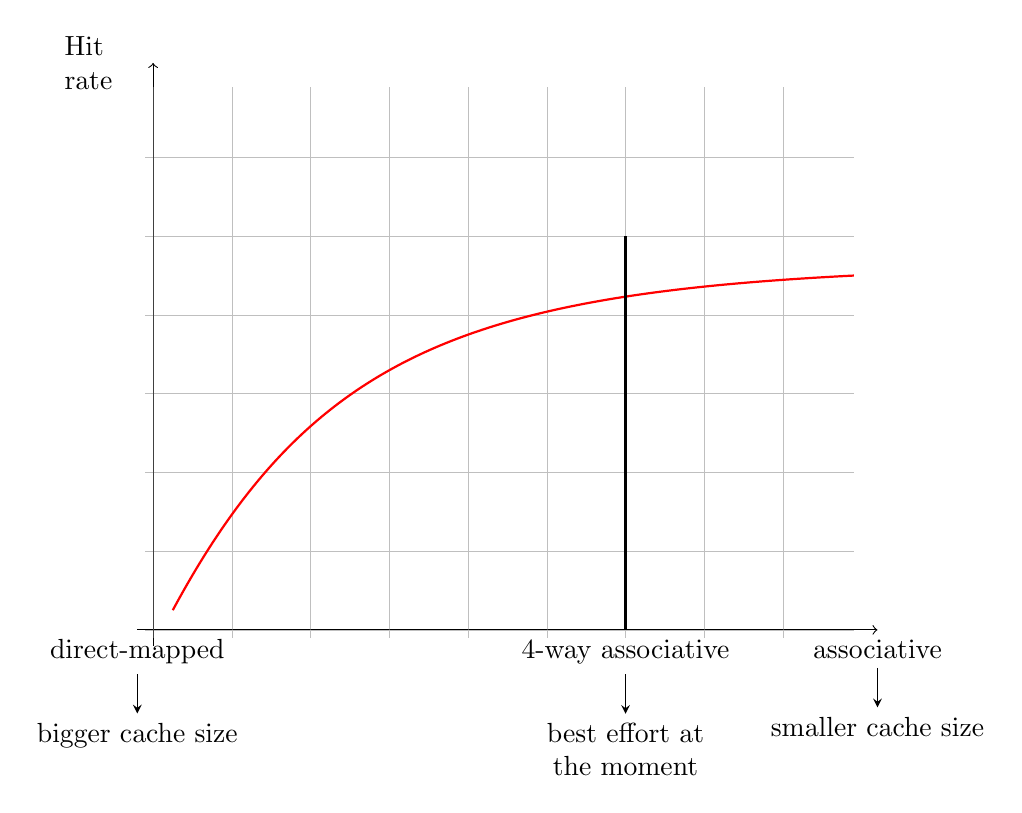
\begin{tikzpicture}
					\draw[->] (-0.2, 0) node[below] (direct_mapped_t) {direct-mapped} -- (9.2, 0) node[below] (associative_t) {associative};
					\draw[->] (0, -0.2) -- (0, 7.2) node[left, text width = 1cm] {Hit rate};
					\draw[very thin, color = gray, opacity = 0.5] (-0.1, -0.1) grid (8.9, 6.9);

					\draw[color = red, thick] (0.25, 0.25) .. controls (2, 3.5) and (4, 4.25) .. (8.9, 4.5);
					\draw[thick] (6, 0) node[below] (4_way_associative_t) {4-way associative} -- (6, 5);
					\draw[->, >=stealth] (direct_mapped_t.south) -- ++(0, -0.5) node[below] {bigger cache size};
					\draw[->, >=stealth] (4_way_associative_t.south) -- ++(0, -0.5) node[below, text width = 2cm, text centered] {best effort at the moment};
					\draw[->, >=stealth] (associative_t.south) -- ++(0, -0.5) node[below] {smaller cache size};
				\end{tikzpicture}
				\caption{Hit rate of different cache designs}
				\label{fig:hitratediffcachedesigns}
			\end{figure}
		}
	}
	\par{
		\noindent\underline{Fragmentation:}
		\par{
			\noindent
			Caused by allocation and deallocation in different order. A bump pointer allocation is performed, the allocated memory is contiguous aligned.
			\begin{figure}[H]
				\centering
				\begin{tikzpicture}
					\tikzset{snake it/.style = {decorate, decoration={snake, amplitude = 6mm, segment length = 10mm}}}

					\node[draw, minimum height = 4cm, minimum width = 2cm] at (0, 2) (nomemhole_node) {};
					\path[draw, snake it, ->, >=stealth] (0, 3.75) -- (0, 0.25);

					\node[draw, minimum height = 4cm, minimum width = 2cm, right = 1 of nomemhole_node.east] (memhole_node) {};
					\path[draw, snake it, >=stealth] (3, 3.75) -- (3, 2.25);
					\path[draw, snake it, ->, >=stealth] (3, 1.25) -- (3, 0.25);
					\draw[->, >=stealth, dashed] (5, 1.75) node[right] {hole} -- (3, 1.75);
				\end{tikzpicture}
				\caption{Memory hole}
				\label{fig:memhole}
			\end{figure}
		}
		\par{
			\noindent\underline{3 solutions:}
			\parskip0pt\begin{enumerate}
				\item{
					Compaction: \newline
					Make bigger holes and get a bound on fragmentation. \newline
					Moving memory in space is slow ($O(n)$ in the size of the memory to move). \newline
					Furthermore the addresses change ($O(n)$ in the size of the memory).
				}
				\item{
					Coalescing: \newline
					Non-moving, merge contiguous free blocks. No bound and causes an improvement on average but not in the worst case.
				}
				\item{
					Partitioning (Prepartitioning): \newline
					\textit{scalloc} implementation from the University of Salzburg (scalable allocation).
				}
			\end{enumerate}
		}
	}
	\par{
		\noindent\underline{scalloc:}
		\begin{figure}[H]
			\centering
			\begin{tikzpicture}
				\def\memoryparth{3cm}
				\def\memorypartw{4cm}
				\tikzset{memory_part/.style = {draw, minimum width = \memorypartw, minimum height = \memoryparth}}

				\node[draw, minimum height = 7.5cm, minimum width = 14cm] at (0, 0) (memory) {};

				\node[memory_part, below right = 0.5 of memory.north west] (memory_part1) {};
				\draw (memory_part1.south) ++(-0.7, 0) -- ++(0, \memoryparth);
				\draw (memory_part1.south) ++(0.7, 0) -- ++(0, \memoryparth);
				\draw (memory_part1.west) ++(0, -0.5) -- ++(\memorypartw, 0);
				\draw (memory_part1.west) ++(0, 0.5) -- ++(\memorypartw, 0);
				\node[draw, circle, below right = 0.55 and 0.725 of memory.north west] (memory_part1_circle1) {X}; 
				\node[draw, circle, below right = 0.55 and 2.1 of memory.north west] (memory_part1_circle2) {X};
				\draw (memory_part1_circle1) -- ++(3, 0) -- ++(0, -1) -- ++(-3, 0) -- ++(0, -1) -- ++(3, 0);

				\node[memory_part, right = 0.5 of memory_part1.east] (memory_part2) {};
				\draw (memory_part2.south) -- (memory_part2.north);
				\draw (memory_part2.east) -- (memory_part2.west);
				\node[draw, circle, below right = 0.5 and 0.65 of memory_part2.north west] (memory_part2_circle) {X};

				\node[memory_part, right = 0.5 of memory_part2.east] (memory_part3) {};

				\node[memory_part, below = 0.5 of memory_part1.south] (memory_part4) {};
				\node[memory_part, below = 0.5 of memory_part2.south] (memory_part5) {};
				\node[memory_part, below = 0.5 of memory_part3.south] (memory_part6) {};

				\draw[<-, >=stealth] (memory_part1.west) ++(0.25, 0) -- ++(-1, 0) node[left, text width = 2cm] {\footnotesize{all of the same size}};
				\draw[<-, >=stealth] (memory_part1.south west) -- ++(-0.75, -1) node[below left, text width = 2.25cm] {\footnotesize{bump pointer allocation inside; spatial locality}};
				\draw[<-, >=stealth] (memory_part1_circle1.north) -- ++(0, 0.75) node[above, text width = 2cm] {\footnotesize{12 byte}};
				\draw[<-, >=stealth] (memory_part2_circle.north) -- ++(0, 1) node[above, text width = 2cm] {\footnotesize{bigger}};
				\draw[<-, >=stealth] (memory_part2.north east) -- ++(0, 0.75) node[above, text width = 3.5cm] {\footnotesize{size-class; when empty can be resized}};
			\end{tikzpicture}
			\caption{Visualization of the \textit{scalloc} idea}
			\label{fig:scallocidea}
		\end{figure}
		
		\noindent \underline{Pros:}
		\parskip0pt\begin{itemize}
			\item{no external fragmentation}
 		\end{itemize}
 		
 		\noindent \underline{Cons:}
 		\parskip0pt\begin{itemize}
 			\item{internal fragmentation (whenever partitioning is done)}
			\item{anything bigger than the partition size cannot be allocated (bound on max. size)}
 		\end{itemize}
	}
}